\pagenumbering{arabic}
\chapter{Introduction}
\label{intro}
The chapter outlines an introduction to the subject area of this Final year Project (FYP), the objectives of this project, the methodology used to complete this project, an overview of the report and an explanation of the motivation behind this FYP.

\section{Overview}
This project explores identification and classification of food images for use in a nutritional assessment android application.
Food calorie consumption is a huge problem in the modern world.
Over 25\% of the population in Ireland is obese and this figure is likely to rise over the coming years.
There has been extensive research carried out into nutritional assessment.
Many of these studies utilise smart phone applications to record calorie intake while physical food diaries have also been used in the past.
A study was carried out by \parencite{goodman2015vitamin} whereby they used a mobile application to keep track of Vitamin D intake for young Canadians ranging from teenagers to early adulthood.
\parencite{arens2015promising} also carried out a review of current computer supported nutritional assessment applications. They applications ranged from web-based applications to smart phones.
The problem with many of these 'food diary' applications is that they can be very tedious and time intensive for users.
Leveraging artificial intelligence to decrease the effort of the user or dietician would be very beneficial and many even encourage use of said nutritional assessment applications.
Artificial intelligence could be utilised to classify food images and calculate the calorie count of an image so that a user would not have to input the information themselves.

The classification of images is the process whereby an algorithm predicts what objects are in an image.
As humans, we take vision for granted.
Computers (which find what are complex task for us, seemingly simple i.e mathematical computations) find it very difficult to interpret images.
A black and white image is simply an array of numbers with values of 1 or 0 as seen in Figure \ref{fig:imageArray}. 
For colour images, there are multiple layers of arrays for each of three colour channels red, green and blue.
It can be quite difficult to extract feature information from these arrays.

\begin{figure}[h]
	\centering
	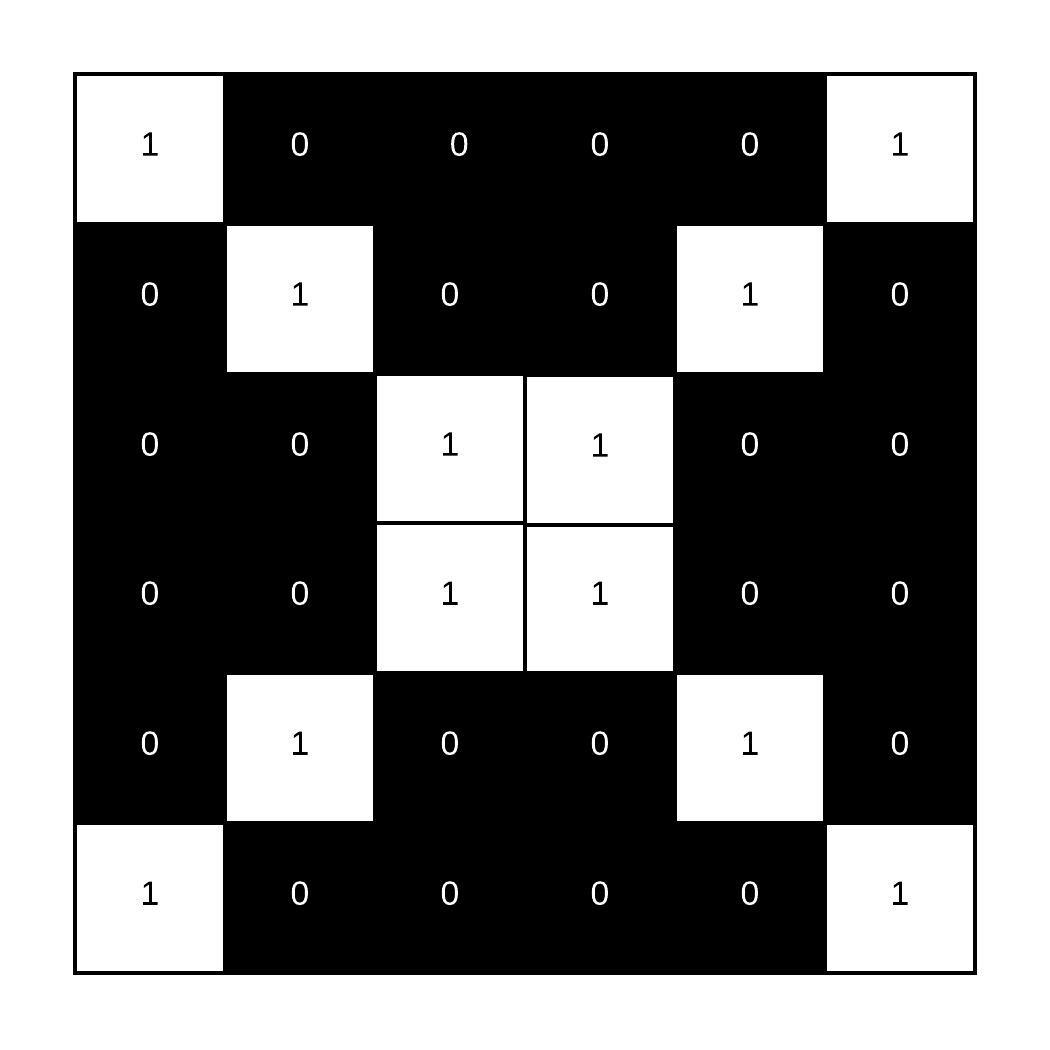
\includegraphics{imageAsArray}
	\caption{Representation of an Image as an Array}
	\label{fig:imageArray}
\end{figure}

Even when classification can be achieved by analysing these arrays of numbers, it is most successful when the object in question takes up most of the image.
For example, the banana is clearly a very prominent object in Figure \ref{fig:bananaClear}.

\begin{figure}[h]
  \centering
	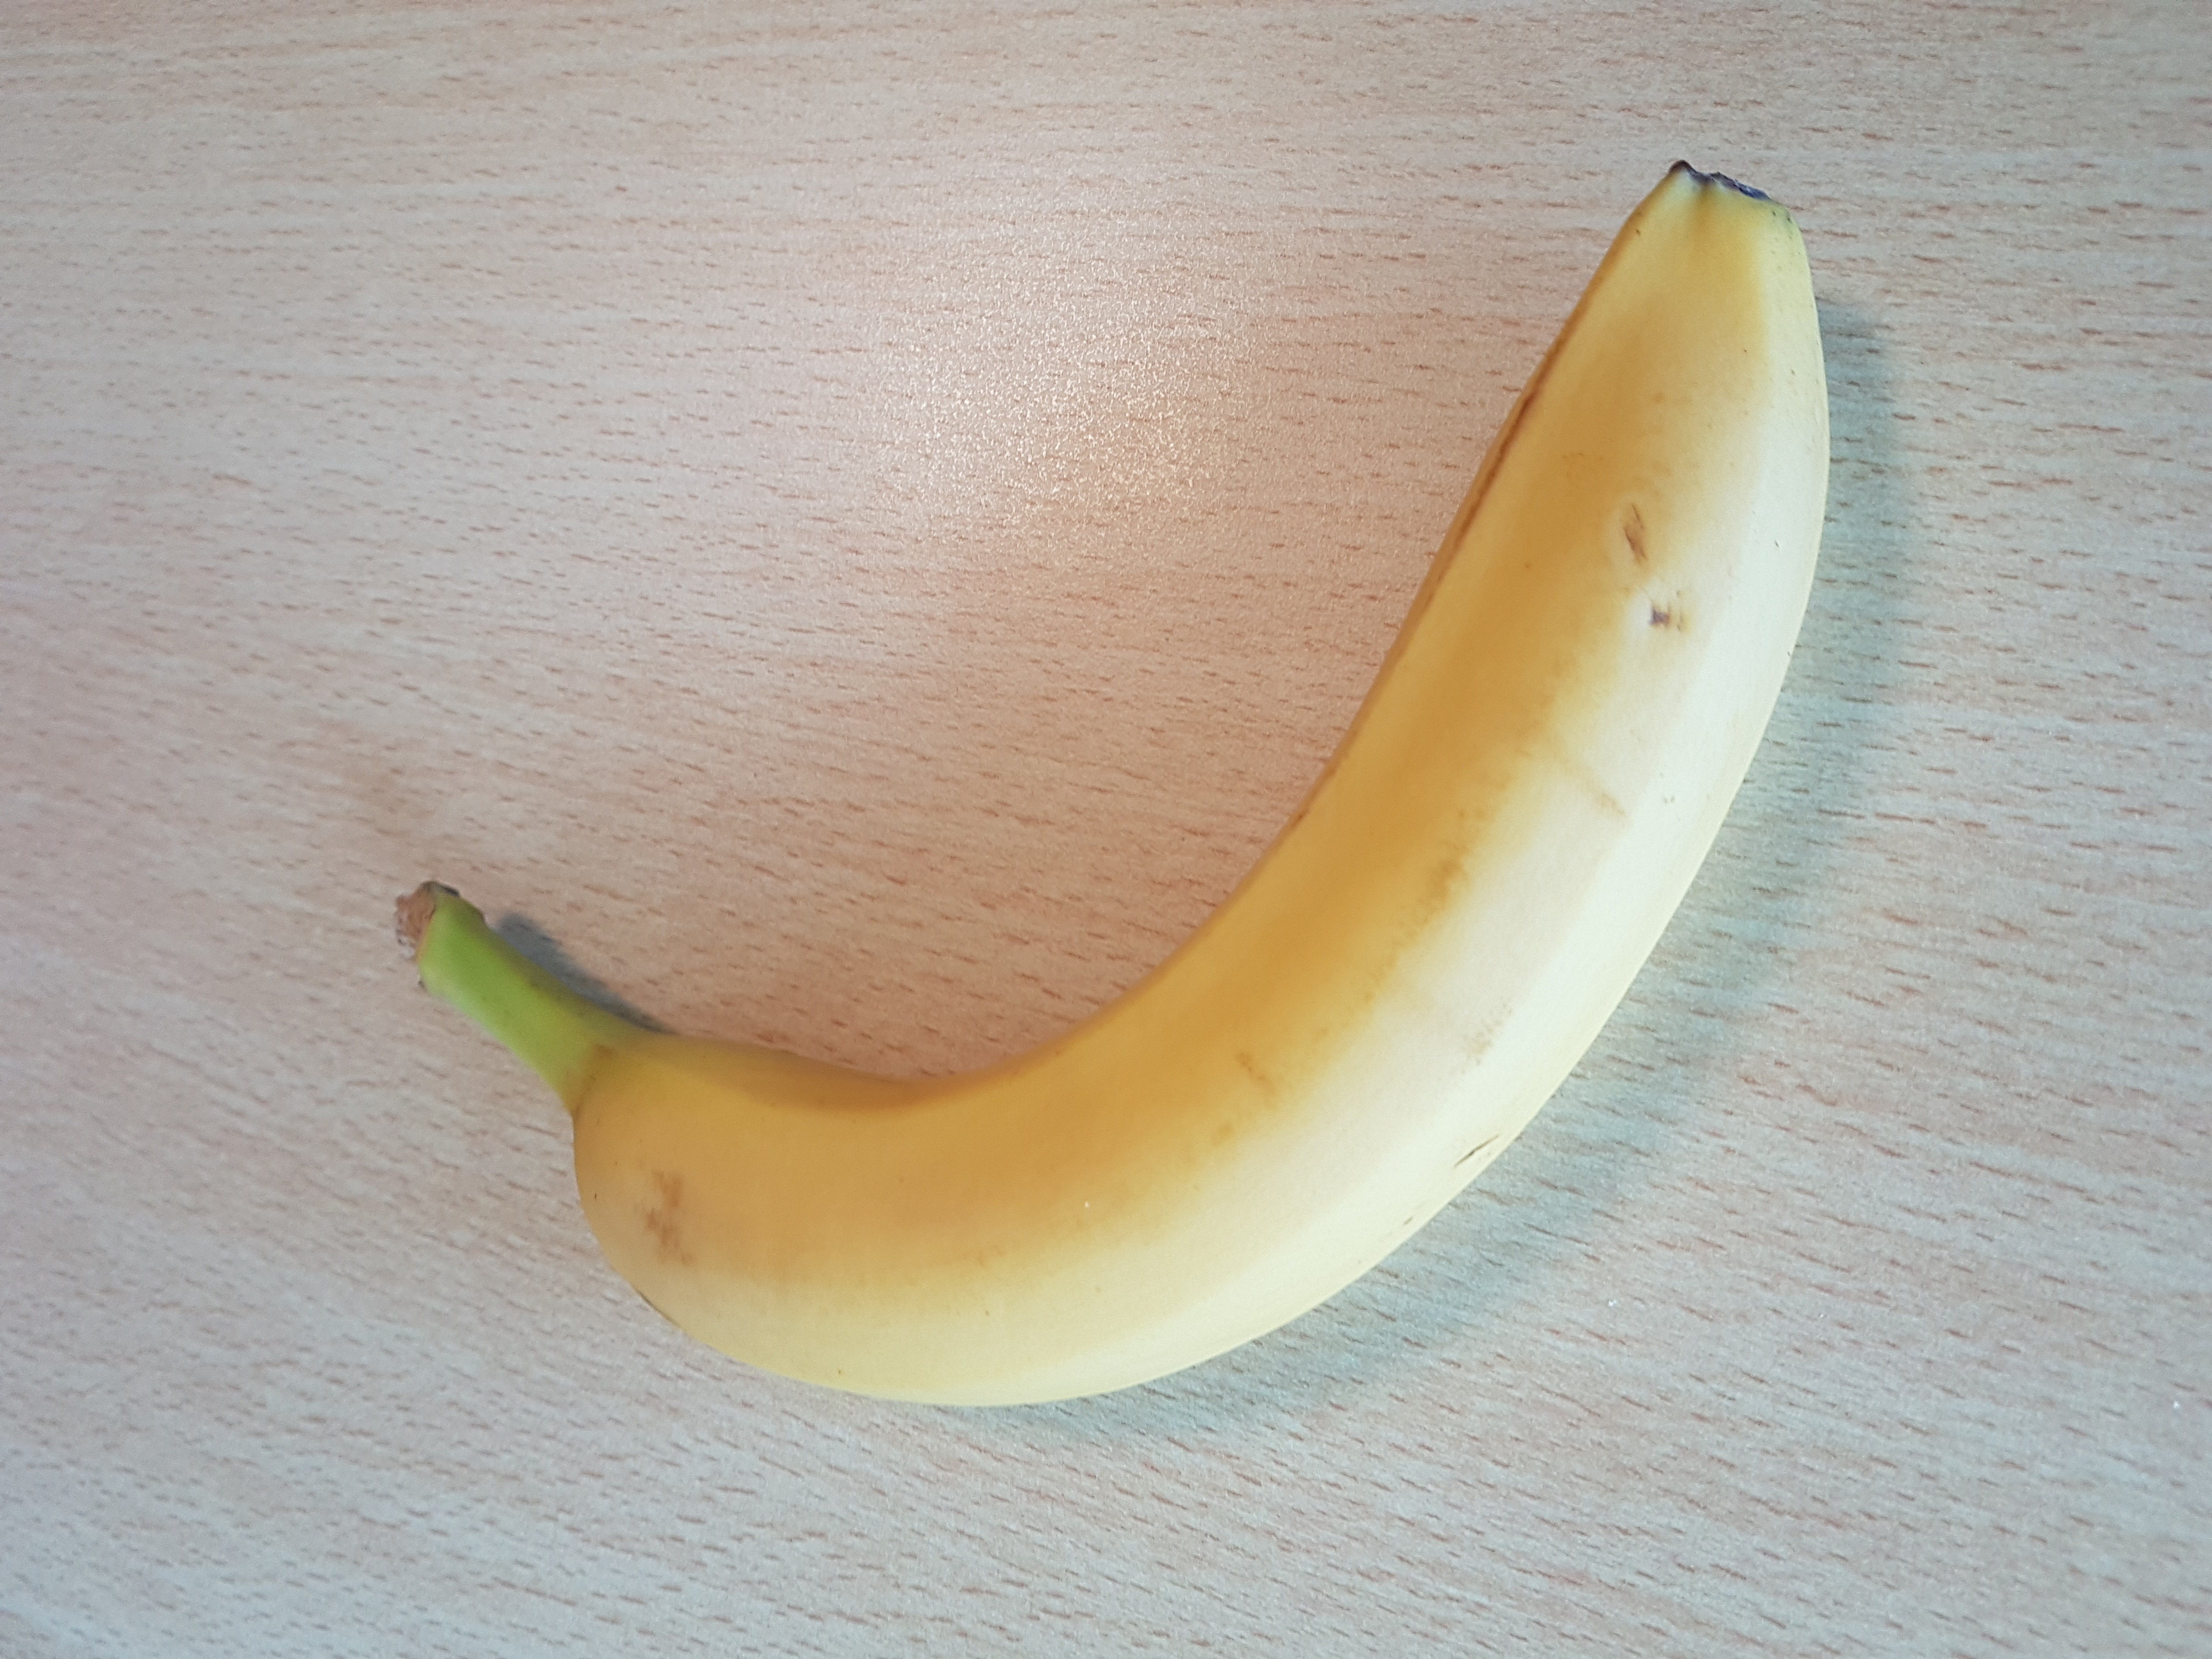
\includegraphics[scale=0.07]{bananaClear}
	\caption{Banana}
	\label{fig:bananaClear}
\end{figure}

Alternatively, when the object of the image is occluded or not the focus of the image (Figure \ref{fig:occludedBanana} and Figure \ref{fig:farBanana}), classification becomes very difficult.
In contrast it can be clearly seen to humans that a banana is still present in both images.
If we take a filled roll for example, it is difficult for the human eye to see the contents never mind a computer so this is another issue that arises.
Illumination is also a factor that influences classification greatly as colour can play an important aspect in classification of food images as discovered by \parencite{novelSVM}.
Other factors of illumination that affect classification are shading, shadows and specular highlights \parencite{dynamicGong}.

\begin{figure}[h] 
  \label{ fig7} 
  \begin{minipage}[h]{0.5\linewidth}
    \centering
    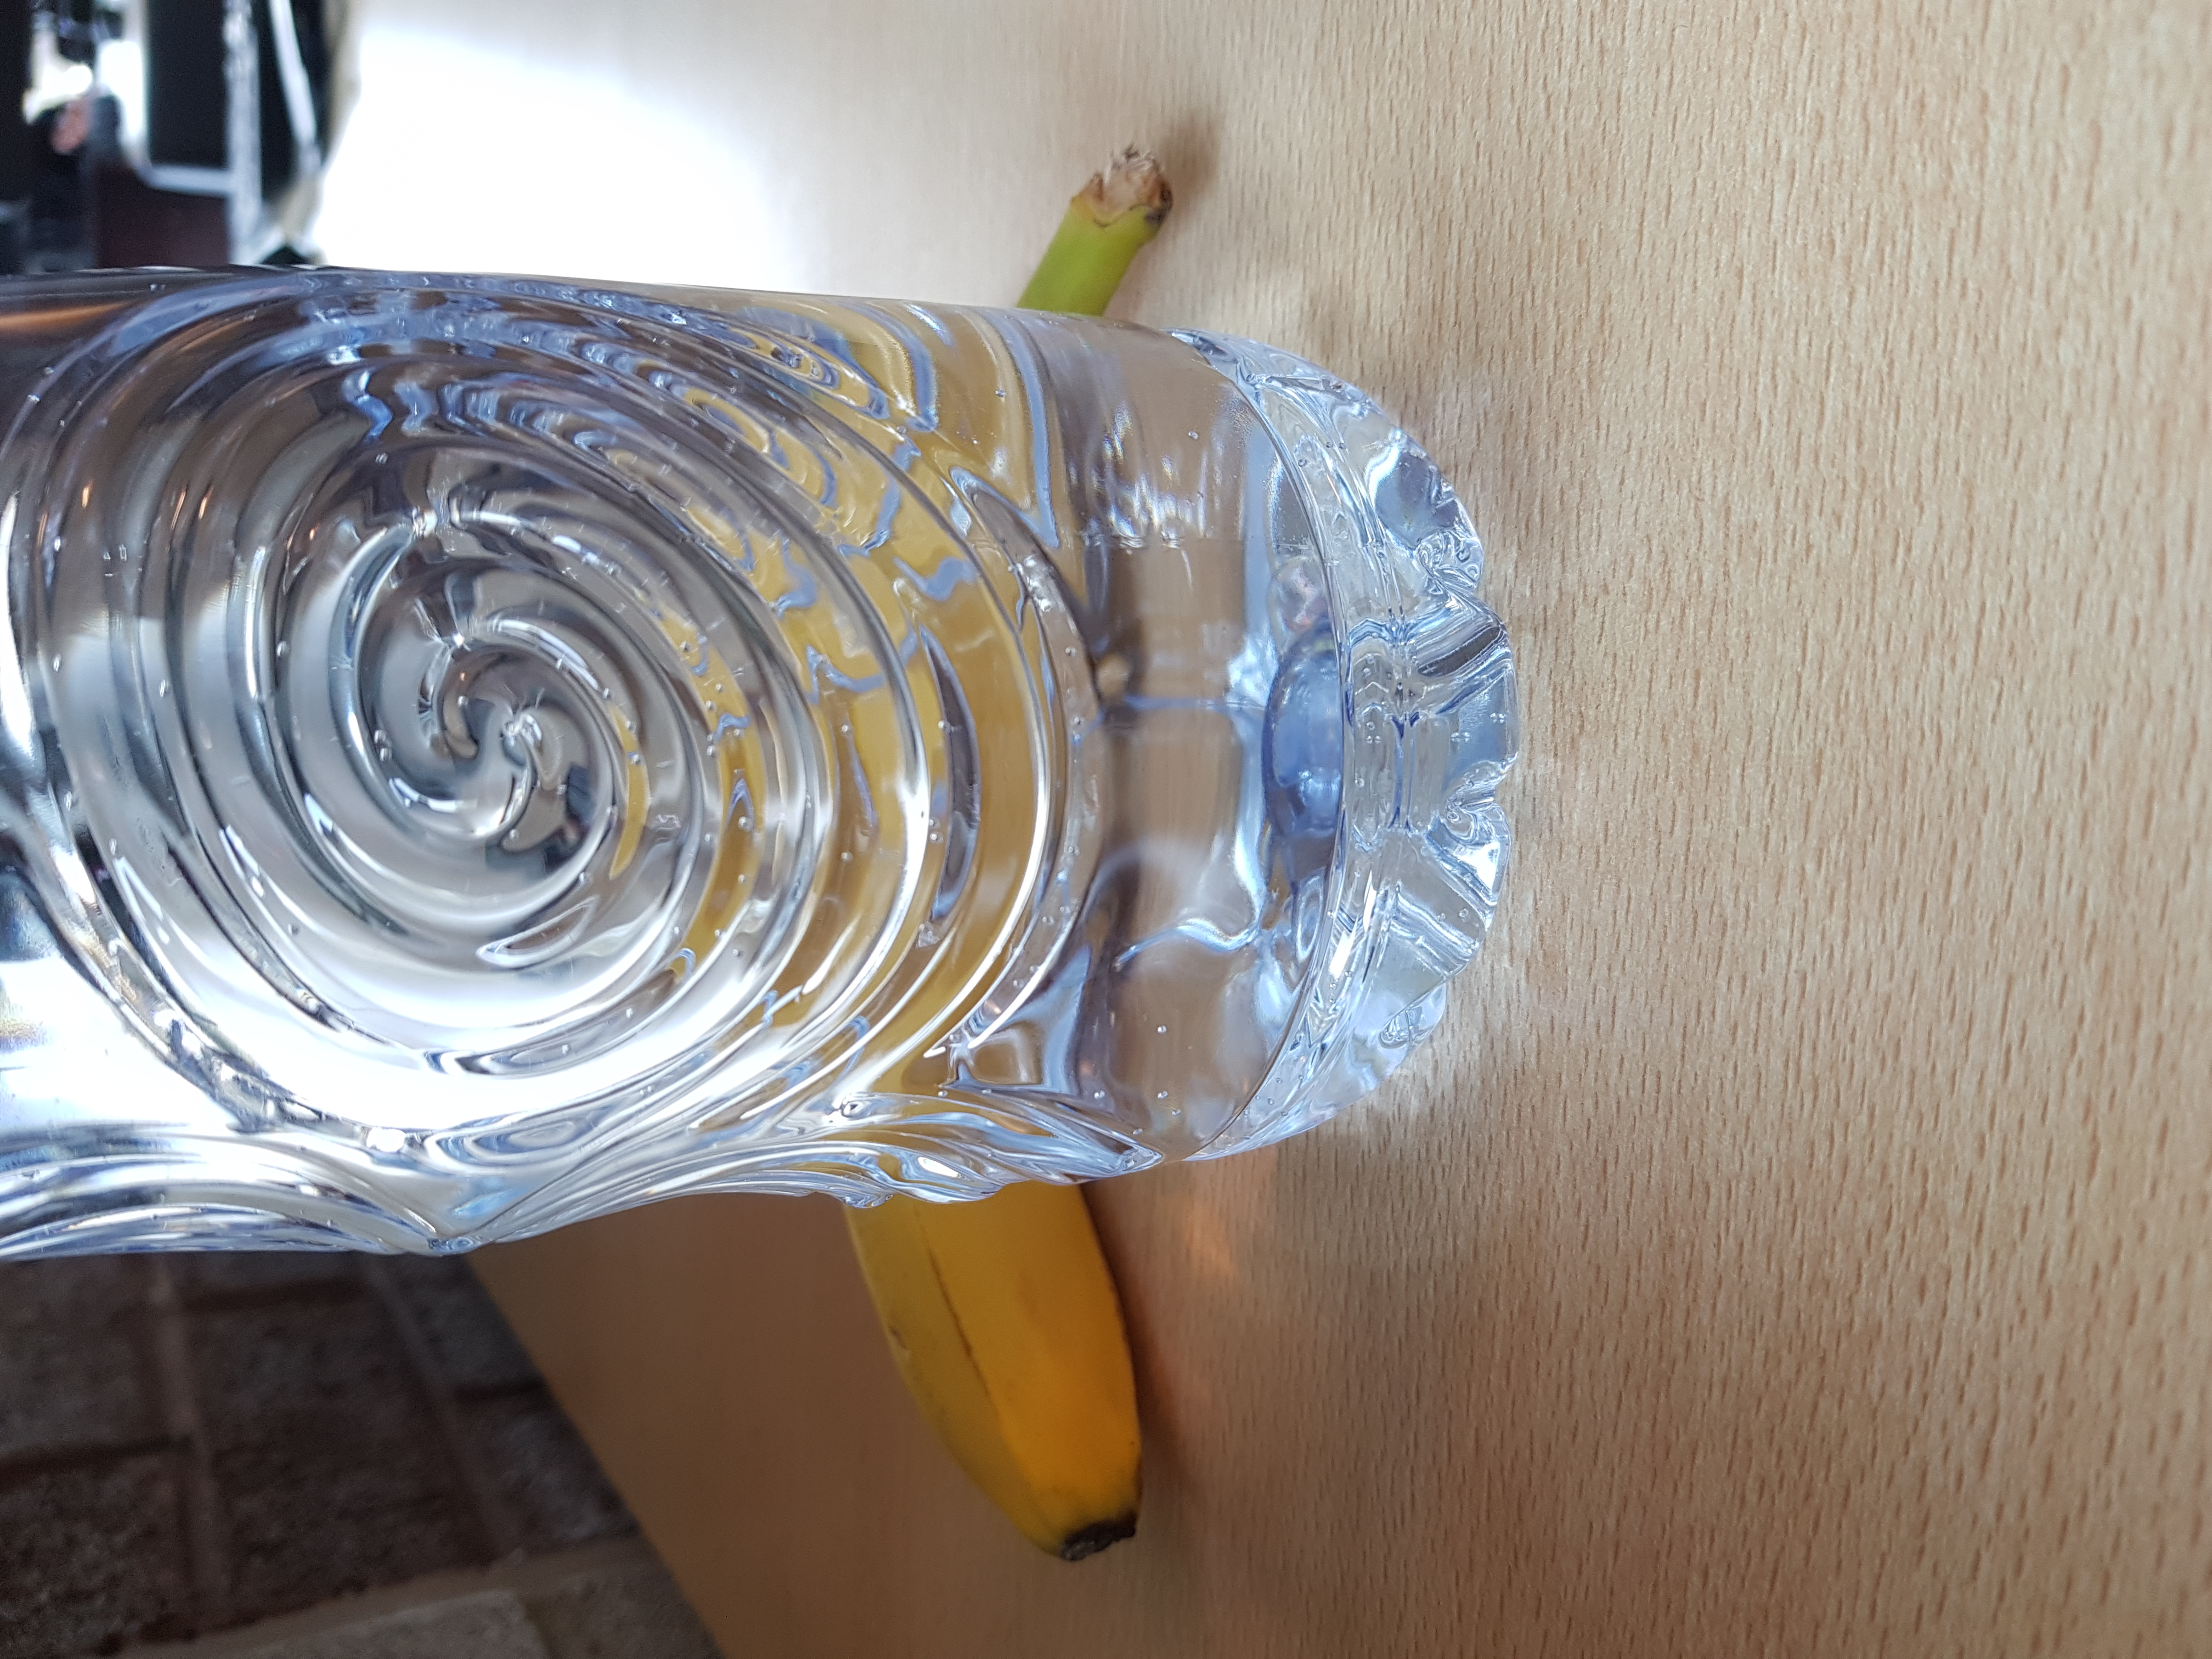
\includegraphics[scale=0.045]{bananaOccluded} 
    \caption{Occluded Banana Image} 
  \label{fig:occludedBanana}
    \vspace{4ex}
  \end{minipage}%%
  \begin{minipage}[h]{0.5\linewidth}
    \centering
    \includegraphics[scale=0.045]{bananaFar} 
    \caption{Banana at Small Scale} 
  \label{fig:farBanana}
    \vspace{4ex}
  \end{minipage} 
\end{figure}

Traditionally, Support Vector Machines (SVMs) have been used to classify food images, many examples of which are covered in Chapter 2.
The aim behind SVMs is to cast the information to a higher dimension, for
example from a 2D to 3D space, so that the classes can be separated. SVMs will be explored further in Chapter 2.
The features used by SVMs for food image classification are normally colour, texture, shape and size as in \parencite{pouladzadeh2014measuring} and \parencite{novelSVM}.
SVMs have their problems however and these problems of long training times and low accuracy with many classes have resulted in SVMs losing popularity in recent years.

Another reason for the shift from the use of SVMs is due to the recent success of utilizing neural networks for image classification.
Neural networks are bio-inspired algorithms based off the structure of the human brain.
A special type of neural networks, Convolutional Neural Networks (CNNs), have proven to be very successful in image classification \parencite{krizhevsky2012imagenet}.
CNNs differ from other neural networks due to their extra layers of convolution and pooling \parencite{visualizing}.
Convolutional layers filter the images for features while pooling refines the information in the arrays to reduce computational time and to make the features in the image clearer.
CNN's have been around since the 1980's \parencite{handsOnML} but were not used by many until 2012 when CNNs became popular again due to the work carried out in that time, for example by \parencite{krizhevsky2012imagenet}.
CNNs have been proven to be very successful in facial recognition and have been applied to food images with promising results as outlined in various studies in Chapter 2 such as \parencite{yanaiFood} and \parencite{deepLearning}.

For a nutritional assessment application, aided by computer vision, there are a
few steps that must completed. Firstly, the food images are classified with prior segmentation in some cases.
Image segmentation is the process by which an image is segmented into multiple parts with usually a segment for each different object or as in the case of Figure \ref{fig:foodSegment} each different food item.
Secondly, size estimation of each food type is carried out. Once data on the food type and size has been collected, calorie count estimation can be undertaken. Size and calorie estimation is outside the scope of this FYP.

\begin{figure}[h]
  \centering
  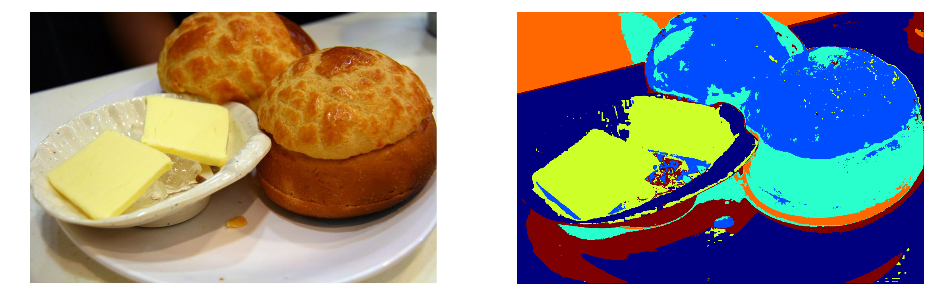
\includegraphics[scale=0.45]{foodSegmentation}
  \caption{Segmented Food Image \parencite{segmentFood}}
  \label{fig:foodSegment}
\end{figure}


The full system proposed to solve the problem statement would be able to integrate with an Android mobile phone application.
The concept is, that when a user is about to eat their meal, they can simply take a picture of their meal for computation.
The application would take an image, and send it to a server to be analysed.
On the server side the image would be classified using a TensorFlow model.
TensorFlow is a machine learning library that can be used to create CNNs.
Once the classification step is completed, the size of each food type would be measured and through this, an overall calorie count would be displayed for the user.
This could be logged for user metrics.
The full system may not be possible to implement due to time constraints so therefore, classification will be the furthest step looked in to.

\section{Objectives}
\subsection*{Primary Objectives}
\subsubsection*{Use Convolutional Neural Networks for Food Image Classification}
There has been a large paradigm shift in food image recognition in recent years to using convolutional neural networks. This paradigm will be used to answer the problem statement.

\subsubsection*{Tune the CNN, replicating previous work}
There are many different approaches to food identification and classification,
many of which we will see in Chapter 2. An approach will be selected that has
shown promising results in the past and replication of these results will be attempted. In addition to this, there are many different network architectures and parameters that can be adjusted when building CNNs and these will be tuned to get the best outcome possible.

\subsubsection*{Develop a mobile application to leverage the CNN}
Another objective for this project is to develop an application that can be used
for dietary assessment. This application would be able to take an image and then send the image to a server to identify and classify the foods within the image. Size estimation will not be explored for this project. Alternatively, due to time constraints, a previously developed application could be used to demonstrate the CNN developed.

\subsection*{Secondary Objectives}
\subsubsection*{Understanding of Convolutional Neural Networks}
In the project, Convolutional Neural Networks (CNNs) will be used for object identification in Food Images.
A machine learning library will be used for this due to time constraints, but it is a key
objective to develop a deep understanding of CNN's as they are quite pivotal in the current computer vision industry and bio-inspired systems are very interesting.

\subsubsection*{Learn about different image identification and classification techniques}
Although, CNN's will be used for implementation, other methods of identification and classification will not be ignored.
It is very important to learn about other methods as different methods
are better suited for some situations and it would be best to know about these methods due to the inevitability of their use.

\section{Contribution}
While many researchers have explored the topic of food image classification, there has not been many comprehensive surveys of the work done.
In Chapter 2 of this report, over 20 research papers have been summarised and critiqued.
This survey of the literature could be very useful for future researchers. 

\section{Methodology}
The following methodology were adapter for this project:

\subsection*{Define the research question}
The first step to this project was to define the research question.
The general area of a computer vision supported nutritional assessment application was known at conception but the scope of this is too broad for an FYP.
Therefore, it was decided that the research question would be to look at the food identification and classification aspect.

\subsection*{Literature Review}
Once the research question was defined, finding related work was the next milestone.
There are many attempts at Food Image Classification and these were not difficult to find, using Google Scholar, but many of these papers glossed over the segmentation aspect and relied on third parties for this step.
Because of this, quite a few references to different papers had to be followed that focused solely on image segmentation and classification.

\subsection*{Explore different image identification methods}
Various image identification methods were collected from the literature review
that was carried out, so there were many options to evaluate.
Convolutional Neural Networks were the clear choice due to recent popularity and successful results, so more traditional methods of identification using colour and texture was not so strenuously explored.

\subsection*{Select an image identification and classification method}
After the various methods to identify and classify food images had been collated in the literature review, one of these had to be selected.

\subsection*{Research technologies and develop skills in these technologies}
As Convolutional Neural Networks (CNN) are used in this project, many resources have been leveraged to enrich understanding of the process.
TensorFlow is the main resource utilised in creating a CNN and on-line tutorials for this technology were greatly beneficial.
A Deep Learning Course on Udacity was also used to enhance understanding and skills.

\subsection*{Build a prototype of the application}
A prototype application had to be built for demonstration for this project.

\subsection*{Compare and analyse results to other implementations}
Once a model had been successfully trained, comparison to previous work was carried out.

\section{Project Plan}

\section{Overview of Report}

This report is broken down into various chapters.
The introduction chapter is to give on overview of what this project is about, how the project will be approached and why it is being carried out.
Following this, some information on the background of the subject of this Final Year Project (FYP) will be outlined. Once the chapters of introduction and background have been completed, a chapter outlining the learning of TensorFlow will be explored. TensorFlow is a machine learning library that is used to develop CNNs. In this chapter, the goal is to demonstrate the activities undertaken to learn about the technologies used and show tutorials that have been completed to aid with this learning.
In chapter titled 'Training Using the Inception-V3 Model Architecture' , the purpose is to outline experiments that have been carried out in relation to training TensorFlow models.
A TensorFlow model is the term used to describe the neural network produced by TensorFlow. 
The Inception-V3 architecture is proven to be a very successful architecture for classifying images and will be explained in detail in said chapter.
Once the model has been trained, the following chapter 'Analysing the Trained Model' will consist of experiments that analyse and test the models trained.
A prototype smart phone application was developed to demonstrate the efficacy of the system and an overview of the process will be explained in the chapter titled 'Prototype Application.'
The final chapter's purpose is to provide a discussion on the results obtained and offer a conclusion to the findings.

\section{Motivation}
I find the topic of Computer Vision a very interesting one.
It excites me, to be able to 'teach' a machine how to see as we do.
For this reason, I really wanted to learn about Neural Networks
and this was a large motivator for this project.

Once I had a topic that I wanted to research, I needed a focus or problem statement for this research.
I find that it is much more rewarding to work on something that positively
impacts both myself and other people, so I decided that I wanted to research
something that fit this requirement.

Food calorie consumption is a very big problem in the modern world.
Over 25\% of the population in Ireland are obese.
A mobile application that could help keep track of a user's calorie intake by taking a picture of their meals would be a big help to combat this problem.
This problem statement works very well for me because of its application use and because of its complexity.
Identifying and recognising food is much more difficult than say recognising faces as it has no uniform shape.
Therefore, this problem would also be very beneficial to developing skills in the computer vision area.

I would like to develop these real-world skills so that I can partake in
Computer Vision projects in industry or to do further research in academia.
I have also been offered a graduate role in Jaguar Land Rover and these skills
would be very relevant in the autonomous driving industry.
This is because machine learning has really taken off in the last few years and is
used by many in industry. While machine learning has become very
popular, computer vision is probably the most prominent that has come out of it.
Face detection, for one, is being researched extensively for use in personalised
advertising and secure access to devices and systems.
